\section{ОБЗОР ЛИТЕРАТУРЫ}
\label{sec:domain}

\subsection{Обзор существующих аналогов}
\label{sub:domain:analogs}

\subsubsection{Windows Toop Help}
\label{sub:domain:analogs:windows}

Одним из интерфейсов получения информаци о процессах и потоках в операционной
системе Windows является библиотека Tool Help\cite{tool_help_article}. Ядром
библиотеки является поняние снимка. Снимок является копией только для чтения
одного или нискольких списков, находящихся в системной памяти:
процессы, потоки, модули и кучи.

Процессы, использующие функции Tool Help, получают доступ к этим спискам из
моментальных снимков, а не непосредственно из операционной системы.
Непосредственно сами списки в системной памяти постоянно изменяются, когда
процессы запускаются и завершаются, потоки создаются и уничтожаются, исполняемые
модули загружаются и выгружаются из системной памяти, а кучи создаются и
уничтожаются. Использование информации из снимка предотвращает несоответствия и
гонки. В противном случае изменения в списке могут привести к тому, что поток
будет неправильно перемещаться по списку или вызвать General Protection Fault.
Например, если приложение обходит список потоков, когда другие потоки создаются
или завершаются, информация, которую приложение использует для перемещения по
списку потоков, может устаревать и может вызвать ошибку для приложения,
перемещающегося по списку.

Снимок создаётся вызовом \texttt{CreateToolhelp32Snapshot}. Он имеет слудующее
определение\cite{win_tool_help}:

\medskip
\begin{lstlisting}[style=cstyle]
HANDLE WINAPI CreateToolhelp32Snapshot(
  _In_ DWORD dwFlags,
  _In_ DWORD th32ProcessID
);
\end{lstlisting}
\medskip

Предоставляется возможным управление содержимым снимка, указав одно или
несколько следующих констант в параметре \texttt{th32ProcessID} при вызове
функции:
\begin{itemize}
\item \texttt{TH32CS\_SNAPHEAPLIST};
\item \texttt{TH32CS\_SNAPMODULE};
\item \texttt{TH32CS\_SNAPPROCESS};
\item \texttt{TH32CS\_SNAPTHREAD}.
\end{itemize}

Флаги \texttt{TH32CS\_SNAPHEAPLIST} и \texttt{TH32CS\_SNAPMODULE} применими при
получении информации об одном процессе. Когда эти значения указаны, списки кучи
и модулей указанного процесса включаются в снимок. При передаче нуля в качестве
идентификатора процесса, используется текущий процесс. При передаче флага
\texttt{TH32CS\_SNAPTHREAD} всегда создается общесистемный снимок, даже если
передан валидный идентификатор процесса.
Для получения состояния куч или модулей всех процессов, передаётся флаг
\texttt{TH32CS\_SNAPALL} и идентификатор текущего процесса. Затем для каждого
дополнительного процесса в снимке снова необходимо вызывать функцию
\texttt{CreateToolhelp32Snapshot} с указанием его идентификатора и флаг
\texttt{TH32CS\_SNAPHEAPLIST} или \texttt{TH32CS\_SNAPMODULE}.

При прохождении по списку процессов используется внутренний итератор. Для
получения информации о первом процессе в списке, используется функция
\texttt{Process32First}. Для дальнейшего перемещения по списку процессов для
последующих записей используется функция \texttt{Process32Next}. Обе функции
заполняют структуру \texttt{PROCESSENTRY32} информацией о процессе в из снимка.
Структура \texttt{PROCESSENTRY32} имеет следующее определение:

\medskip
\begin{lstlisting}[style=cstyle]
typedef struct tagPROCESSENTRY32 {
  DWORD     dwSize;
  DWORD     cntUsage;
  DWORD     th32ProcessID;
  ULONG_PTR th32DefaultHeapID;
  DWORD     th32ModuleID;
  DWORD     cntThreads;
  DWORD     th32ParentProcessID;
  LONG      pcPriClassBase;
  DWORD     dwFlags;
  TCHAR     szExeFile[MAX_PATH];
} PROCESSENTRY32, *PPROCESSENTRY32;
\end{lstlisting}
\medskip

Как видно из определения, предоставленный разработчиками системы интерфейс
позволяет получить такие параметры процесса, как идентификатор, число потоков,
идентификатор родительского процесса, базовый приоритет созданных данным
просцессом потоков, имя исполняемого файла процесса. Четыре поля структуры
больше не используются, что показывает важность и серьёзность построения
интерфейса, по возможности устойчивого к изменениям архитектуры системы, при
которых элементы существующего интерфейса теряют смысл.

\subsubsection{Apple macOS}
\label{sub:domain:analogs:macos}

Несмотря на то, что система macOS является прямым потомком UNIX, она не имеет
собственной реализации \texttt{procfs}. Такие утилиты как \texttt{ps} используют
вместо этого интерфейсы kvm и sysctl\cite{osxproc}. Кроме того, предоставляется
системная библиотека libproc.h, а ныне устаревшие версии macOS для сбора
информации о процессах имели интерфейс Process Manager.

Process Manager ведет список всех открытых процессов\cite{procmanag}. Получение
элементов списка производится вызовами функции \texttt{GetNextProcess}. Такой
интерфейс похож на решение в ОС Microsoft Windows, однако не требует создания
снимка, а в качестве единственного аргумента принимает последний валидный
идентификатор процесса, возвращенный одной из функций % \texttt{GetNextProcess},
\texttt{LaunchApplication}, \texttt{GetFrontProcess}, \texttt{GetCurrentProcess}
или константу \texttt{kNoProcess} в начале хождения по списку. Порядок, в
котором будут предоставляться идентификаторы, жёстко не регламентирован и
является внутренним для Process Manager. Кроме того, полученный идентификатор
процесса можно использовать только в других функциях Process Manager.

Для получения информации о конкретном процессе в Process Manager используется
функция \texttt{GetProcessInformation}. Кроме полученного ранее инденитфикатора
процесса в функцию передаётся указатель на структуру \texttt{ProcessInfoRec}, в
которую будет помещена информация о процессе. Структура имеет следующее
определение:

\medskip
\begin{lstlisting}[style=cstyle]
TYPE ProcessInfoRec =
   RECORD
      processInfoLength:   LongInt;
      processName:         StringPtr;
      processNumber:       ProcessSerialNumber;
      processType:         LongInt;
      processSignature:    OSType;
      processMode:         LongInt;
      processLocation:     Ptr;
      processSize:         LongInt;
      processFreeMem:      LongInt;
      processLauncher:     ProcessSerialNumber;
      processLaunchDate:   LongInt;
      processActiveTime:   LongInt;
      processAppSpec:      FSSpecPtr;
   END;
\end{lstlisting}
\medskip

В структуре водержится, имя и идентификатор процесса, тип и подпись процесса,
адрес раздела с процессом, размер свободной памяти в куче, идентификатор
родительского процесса, время запуска процесса, накопленное процессорное время и
расположение исполняемого файла процесса. Кроме этого, имеются флаги, которые
описывают, является ли процесс приложением или Desk Accessory.

Библиотека libproc.h предоставляет бинарный интерфейс, дающий возможность получать
различную информацию, не привязываясь к внутренним структурам данных, так как
используются либо типы, определённые в стандарте POSIX, либо структуры,
определённые специально только для передачи информации пространству
пользователя\cite{libproc}. Использование библиотеки не требует сохранения
снимка в памяти ядра, что лишает разработчика возможности работать с абсолютно
постоянным списком, но экономит память и предотвращает ситуацию, когда множество
процессов создают так много снимков, что память ядра заканчивается. Определения
некоторых функций:

\medskip
\begin{lstlisting}[style=cstyle]
int	proc_listpidspath(uint32_t	type,
			  uint32_t	typeinfo,
			  const char	*path,
			  uint32_t	pathflags,
			  void		*buffer,
			  int		buffersize);
int proc_listpids(uint32_t type, uint32_t typeinfo,
                  void *buffer, int buffersize);
int proc_listallpids(void * buffer, int buffersize);
int proc_listpgrppids(pid_t pgrpid,
                      void * buffer, int buffersize);
int proc_listchildpids(pid_t ppid,
                       void * buffer, int buffersize);
int proc_pidinfo(int pid, int flavor, uint64_t arg,
                 void *buffer, int buffersize);
int proc_pidfdinfo(int pid, int fd, int flavor,
                   void * buffer, int buffersize);
int proc_pidfileportinfo(int pid, uint32_t fileport,
        int flavor, void *buffer, int buffersize);
\end{lstlisting}
\medskip

Такой подход является более устойчивым к изменениям внутренней архитектуры ядра,
при нём маловероятна ситуация, когда большая часть полей структуры больше нет
смысла использовать, как это произошло с Tool Help в Windows. Кроме того, такие
функции достаточно расширяемы засчёт параметра, определяющего тип результирующих
данных, необходимых пользовательской программе.

\subsubsection{Файловая система \texttt{procfs}}
\label{sub:domain:analogs:procfs}

ФС \texttt{procfs} имеет множество реализаций на разных платформах, впервые
появившись ещё в UNIX V8. По первоначальной задумке должна была предоставляться
информация только о процессах, каждый из которых был представлен своей
директорией в корне относительно точки монтирования. Реализация в Linux
несколько отошла от этого ограничения, фактически дополнительно предоставляя и
более общую информацию о системе, такую как точки монтирования, статистика
планировщика, загруженные модули, версия и загрузочные параметры ядра и
другие\cite{rlove}.

Кроме того, \texttt{procfs} подчиняется пространствам имён согласно UNIX
Timesharing System, а также при монтировании позволяет контролировать количество
доступных данных текущему пользователю. При этом доступ к данным можно разрешить
всем пользователям, сделать данные о других пользователях невидимой либо
разрешить доступ только к своим данным. Данные возможноти позволяют при
необходимости сильнее изолировать процесс, тем самым повышая безопасность
системы.

Каждая описывающая процесс диктория имеет название, явлющееся индентификатором
PID\cite{understanding}. Каждая директория содержит отдельные файлы, содержащие
командную строку 
процесса, переменными окружения, отображениями в память, точками монтирования,
таблицей странц, статистикой планировщика, текущим стеком, общей статистикой и
прочим. Для каждого такого файла необходимо осуществлять как минимум три
системных вызова: \texttt{open()}, множество вызовов \texttt{read()} и
\texttt{close()}, что не может не сказываться на производительности.

Информация о файловых дескрипторах представлена такими директорями как
\texttt{/proc/\$PID/fd/} и \texttt{/proc/\$PID/fdinfo/}. Файлы в директории
\texttt{fd/} представляют собой символьные ссылки с именами~---
номерами дескрипоторов. Ссылки указывают на соответствующие открытые файлы,
устройства, каналы или сокеты. Открытием такой ссылки предоставляется
возможность читать открытый процессом файл, даже если он уже удалён. Индикатором
того, что файл удалён, служит приписка <<(deleted)>> через пробел в конце
строки, получаемой в результате вызова \texttt{readlink()}. Такое решение
допускает возможность введения пользовательской программы в
заблуждение\cite{johnson}, так как
существующий файл также может содержать подобную приписку в названии, ведь
единственные ограничения для имени файла в соответствии со стандартом POSIX~---
отсутствие символов <</>> и <<\textbackslash0>> (разделитеть пути и терминатор
строки в Си), и размер:

\medskip
\begin{lstlisting}[style=cstyle]
# cat /proc/2189/fdinfo/8
pos:    0
flags:  02004002
mnt_id: 13
clockid: 0
ticks: 0
settime flags: 03
it_value: (7700168127, 274769547)
it_interval: (0, 0)
# readlink /proc/2189/fd/8
anon_inode:[timerfd]
# readlink /proc/1329/fd/4
/home/postskript/sec_domain.tex
# rm /home/postskript/sec_domain.tex
# readlink /proc/1329/fd/4
/home/postskript/sec_domain.tex (deleted)
\end{lstlisting}
\medskip

Элементы директории \texttt{/proc/\$PID/fdinfo/} также именуются номерами
дескрипторов, но являются файлами с такой информацией как текущая позиция,
флаги, идентификатор точки монтирвования, а также типозависимые данные.

Ранее уже имели место случаи, когда происводительность программы сильно падала
не без участия \texttt{procfs}\cite{slowperf}. На рисунке \ref{fig:perf_bug}
изображено сообщение о том, как на сервере с почти 30000 процессов запуск
\texttt{perf top} занял около 20 минут. При этом автор отмечает частые обращения
к виртуальной файловой системе.

\begin{figure}
  \centering
  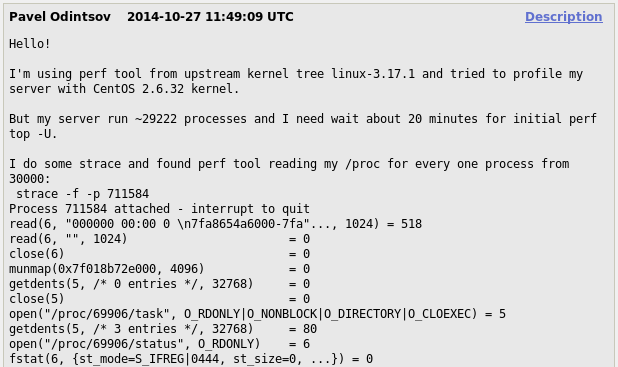
\includegraphics[scale=0.7]{perf_bug.png}
  \caption{Сообщение о низкой производительности в багтрекере ядра \cite{slowperf}}
  \label{fig:perf_bug}
\end{figure}

Продемострировать затратность получения информации из файлов возможно несколькими
способами: посчётом числа и времени в необходимых системных вызовах с помощью
\texttt{strace -c}, и подсчётом времени выполнения необязательных функций
утилитой \texttt{perf}. Кроме того, важно при замере производительности
изолировать процесс от воздействия внешних факторов для повышения точности
измерений. К таким факторам относятся непостоянность частоты ЦП ввиду
автоматического подстраивания её под текущую нагрузку, прерывания, а также
другие процессы на текущем ядре\cite{kernelnewbies}.

В первую очередь, ядро загружается с параметром \texttt{nr\_cpus=1} для нагрузки
по умолчанию только одного ядра процессами\cite{kernel_docs}.
Отключение изменения частоты процессора можно осуществить записью единицы в
виртуальный файл
\texttt{/sys/devices/system/cpu/intel\_pstate/no\_turbo}. Записью в файлы
\texttt{/proc/irq/*/smp\_affinity} разрешается обработка прерываний только на
нулевом процессоре, после чего при утилитой \texttt{taskset} необходимый
процесс запускается на свободном процессоре.

\begin{figure}
  \centering
  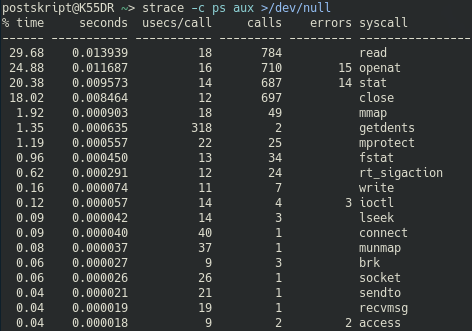
\includegraphics[width=\textwidth]{strace_ps.png}
  \caption{Получение статистики системных вызовов в ps}
  \label{fig:strace_ps}
\end{figure}

На рисунке \ref{fig:strace_ps}
продемонстрирован результат анализа выполнения команды
\texttt{strace -c ps aux}. Полученный результат
показывает, что операции, являющиеся дополнительными действиями из-за работы с
данными через виртуальные файлы и не приносящие никакой полезной информации,
могут занимать до половины времени процесса в пространстве ядра. При этом стоит
учитывать, что полученные таким способом результаты не учитывают временные
затраты на преобразования входных и выходных данных. 

Результат работы профилировщика показан на рисунке \ref{fig:perf_report}.
Итоговый суммарный процент времени на дополнительные расходы равен около 20\%.
На высоконагруженных системах такая разница будет значительной, что и было
показано ранее.

\begin{figure}
  \centering
  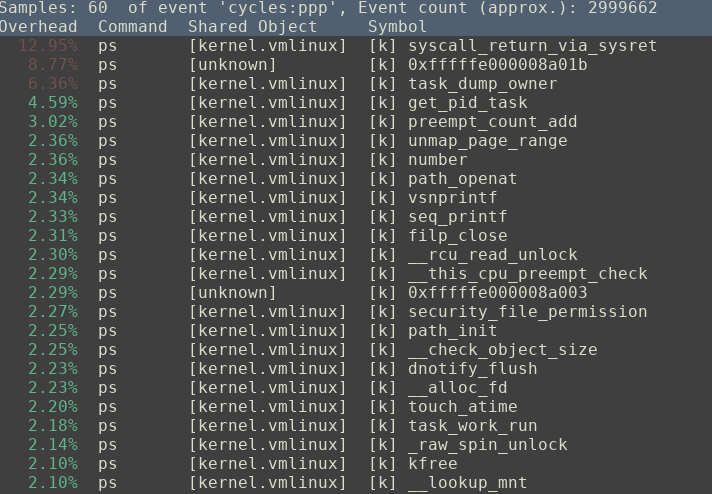
\includegraphics[width=\textwidth]{perf_report.png}
  \caption{Результат анализа производительности}
  \label{fig:perf_report}
\end{figure}

\subsection{Аналитический обзор}
\label{sub:domain:analitic_overview}

С учётом обзора существующих аналогов и выделения их слабых и сильных сторон,
необходимо выделить наиболее важные критерии, соответствующие нынешним
требованиям индустрии:

\begin{itemize}
\item низкая требовательность по памяти;
\item высокое быстродействие;
\item безопасность и надёжность;
\item невозможность пользовательским программам напрямую влиять на объём
  выделенной памяти в пространстве ядра;
\item однозначность интерпретирования полученных данных;
\item стабильность формата без необходимости заглушек.
\end{itemize}

Ранее в среде Linux имела место попытка добавления альтернативного интерфейса
получения системной информации о процессах при помощи интерфейса
Netlink\cite{vagin}. Интерфейс представлял собой дополнительный файл в корне
\texttt{procfs}, взаимодействие с которым осуществляется тому же принципу, что и
с сокетами. Такое решение позволяло несколько ускорить получение данных, однако
всё ещё требовало работы с файловой системой, что снова вызывает накладные
расходы. Кроме того, предложенное решение игнорировало любые пространства имён,
кроме сетевого. Как результат, патчи не были приняты.

Таким образом, оптимальным решением для получения информации о процессах и
файловых дескрипторах является традиционный метод взаимодействия программ
пространства с ядром~--- системные вызовы\cite{man_syscall}. Такое решение
позволит обойтись без использования виртуальной файловой системы, обеспечить
достаточную безопасность, производительность и корректность.

\nocite{tanenbaum, lkml}
